\documentclass{article}

\usepackage[utf8]{inputenc}
\usepackage{mathtools}
\usepackage{listings}
\usepackage{color}
\usepackage{fancyvrb}
\usepackage{tabularx}
\usepackage{fancyref}
\usepackage{enumitem}
\usepackage[margin=0.75in]{geometry}
\usepackage{amsmath}
\usepackage[square,numbers,sort&compress]{natbib}

\title{Molecular Simulation of Materials, Homework 1}
\author{Matthew Grasinger}

\begin{document}

\lstset{language=C++,
        basicstyle=\ttfamily,
        keywordstyle=\color{blue}\ttfamily,
        stringstyle=\color{red}\ttfamily,
        commentstyle=\color{green}\ttfamily,
        morecomment=[l][\color{magenta}]{\#},
        breaklines=true,
        postbreak=\raisebox{0ex}[0ex][0ex]{\ensuremath{\color{red}\hookrightarrow\space}}
}

\pagenumbering{gobble}
\vspace{3.5in}
\maketitle
\clearpage
\pagenumbering{arabic}

\section{Problem 1}

\begin{enumerate}[label=\roman*)]
  \item The polynomial computation was implemented in three templated functions of the signature \texttt{template <typename T> T f(const T)}.
    Each of these three functions are described in \Fref{tab:parti} and the source code is presented in \Fref{sec:src1}.

    \begin{table} \label{tab:parti}
      \caption{Implementations of functions to calculate $2x^4 - 3x^4 + 4x^2 - 3$.}
    \begin{tabularx}{\linewidth}{ r X }
      \textbf{Function name} & \textbf{Description} \\
      \hline & \\
      \texttt{part\_i\_slowest} & Calculates polynomial using the \texttt{pow} function.\\
      \\
      \texttt{part\_i\_fast} & Calculates polynomial by replacing each exponent with the correspond series of multiplications (e.g. $x^6 \rightarrow x*x*x*x*x*x$)\\
      \\
      \texttt{part\_i\_fastest} & Calculates polynomial by: (1) caching the value of $x^2 = x*x$; (2) caching the value of $x^4 = x^2 * x^2$, and (3) calculating the polynomial as: $2*x^4*x^2 - 3*x^4 + 4*x^2 - 3$\\
    \end{tabularx}
  \end{table}

    Theoretically, \texttt{T part\_i\_fast(const T)} and \texttt{T part\_i\_fastest(const T)} should be more computationally efficient than \texttt{T part\_i\_slowest(const T)} because the \texttt{pow} is a computationally expensive method to calculate $x^6$, $x^4$, and $x^2$.
    In addition, if you count the multiplication and division operations, \texttt{T part\_i\_fast(const T)} requires 12 operations and \texttt{T part\_i\_fastest(const T)} only requires 6.
    Therefore, of the three implementations \texttt{T part\_i\_fastest(const T)} should be the fastest.
    
    Each of the three functions were profiled to measure its computation time.
    The results of (1) the return value of each function for each input number, and (2) the associated computation time are presented in the output (\Fref{sec:output1}).
    For every case (i.e. each combination of number and return type), \texttt{part\_i\_slowest} had the most computing time; and in general, \texttt{part\_i\_fastest} required less computing time than \texttt{part\_i\_fast}.
    Therefore, the results were consistent with what one would intuitively expect given that the \texttt{pow} function is computationally expensive, and \texttt{part\_i\_fastest} had the least amount of multiplication operations.
  \item A function was written to determine whether or not an integer is prime, \texttt{bool is\_prime(const int x)}.
    Its implementation is given in \Fref{sec:src1}.
    The algorithm works by:
    \begin{enumerate}
      \item checking to see if $x < 1$.
        If $x$ is zero or negative, it cannot be prime.
      \item checking to see if $x = 1$ or $x = 2$.
        If $x$ is 1 or 2 then it is prime.
      \item checking to see if $x$ can be divided by 2 without remainder.
        If $x$ can be divided by 2 without remainder, and is not 2 (as verified by the previous step), then $x$ is even.
      \item checking each odd number less than $x$ to see if it divides $x$ without remainder.
        Only the odd numbers need to be checked because the previously step accounted for all of the even numbers.
        If an odd number is found to divide $x$ without remainder, then $x$ is not prime.
        Otherwise, $x$ is prime.
    \end{enumerate}
    Although this algorithm is simple, it is theoretically twice as efficient as the brute force approach (checking every positive integer less than $x$ to see if it divides into $x$ without remainder).
    \item There is a clear difference between the polynomial functions that have a return type of \texttt{int} and those that have a return type of \texttt{double}.
     For the smallest numbers, 11 and 28, all of the functions agree.
     However, for the numbers greater than 28 (45, 397, 677, 951, 2552, 6447) the functions with return type \texttt{int} experience numerical overflow (i.e. the computed value is greater than what can be stored).
     This happens because an \texttt{int} is only 4 bytes (on my machine) and a double is 8 bytes.
\end{enumerate}

\pagebreak

\subsection{Source: \texttt{start.cpp}} \label{sec:src1}

{\centering \small
\lstinputlisting{start.cpp}
}

\pagebreak

\subsection{Output} \label{sec:output1}

{\centering \small
\VerbatimInput{5output.txt}
}

\section{Problem 2}

The two papers that are of interest to me, and that have been included in this submission are \textit{Atomistic-to-continuum multiscale modeling with long-range electrostatic interactions in ionic solids}, \citet{marshall2014atomistic} and \textit{Introduction to the Kinetic Monte Carlo Method}, \citet{voter2007introduction}.
I chose \cite{marshall2014atomistic} because I am interested in techniques and computational approaches for multiscale modeling.
I am interested in multiscale modeling because (1) it is a relatively new area of research in numerical methods, (2) it presents challenges that are non-trivial from an analysis, or mathematical standpoint (e.g. proving uniqueness and existance of solutions, well-posedness, etc.), and from a standpoint of computational efficiency and (3) there are many problems in engineering that require information and analysis on multiple scales (e.g. crack initiation at material defects, solid electrolytes that conduct current through the motion of charged point defects, etc.).
The multiscale approach presented in \cite{marshall2014atomistic} uses a lot of the concepts that we have covered in class such as short-range, pairwise, Lennard-Jones potentials, but also addresses other topics such as how to efficiently model long-range potentials such as electrostatic potentials.

My interest in \cite{voter2007introduction}, and the Kinetic Monte Carlo in general, stems from the fact that I find it interesting that the evolution of a physical system can be approximated from random sampling and a few additional constraints.
What is presented in \cite{voter2007introduction} is an overview of different Kinetic Monte Carlo methods with the goal of helping the reader to assess other papers using Kinetic Monte Carlo and to give the reader the basic tools necessary to develop their own Kinetic Monte Carlo application.
As discussed in class, molecular dynamics simulations are typically limited to about a microsecond of simulation time.
It is interesting how Kinetic Monte Carlo methods try to overcome this limitation in time-scale by (often) no longer attempting to follow the exact trajectory of particles through their every vibrational period, but instead focus on dynamics of a coarser time-scale.

\section{Problem 3}

\begin{enumerate}[label=\alph*)]
  \item If we assume the water droplets are at room temperature, $25 \text{ C}$, then the density is approximately $0.997044 \text{ g} / \text{cm}^3$.
    In addition, water molecules are approximately $10 \text{ g} / \text{mol}$, or $10 \text{ g}$ per $6.022 \times 10^{23}$ molecules.
    Using both the density and atomic mass of water, we can obtain:
    \begin{equation} \label{eq:NperV}
      \frac{\rho}{10 \text{ g} / 6.022 \times 10^{23}} = \frac{0.997044 \text{ g} / \text{cm}^3}{10 \text{ g} / 6.022 \times 10^{23}} = 6.004 \times 10^{23} \text{cm}^{-3} = 6.004 \times 10^{2} \text{ nm}^{-3}.
    \end{equation}
    For spherical droplets of diameter $1$ nm, $10$ nm, and $100$ nm, the volume is $\pi / 4 \text{ nm}^3$, $25 \pi \text{ nm}^3$, and $2500 \pi \text{ nm}^3$, respectively.
    Plugging these volumes in \eqref{eq:NperV} results in $471$, $47155$, and $4.7155 \times 10^6$ molecules, respectively.
  \item For each pair of water molecules, there are $9$ distinct pair interactions; and for $N$ molecules, we can choose $\frac{N(N-1)}{2}$ distinct pairs of molecules.
    The number of distinct pair interactions for $N$ molecules is therefore $9 \frac{N(N-1)}{2}$.
    The number distinct pair interactions in a spherical water droplet with diameter $1$ nm, $10$ nm, and $100$ nm are $996165$, $10^{10}$, and $10^{14}$, respectively.
\end{enumerate}

\section{Problem 4}

\begin{enumerate}[label=\alph*)]
  \item 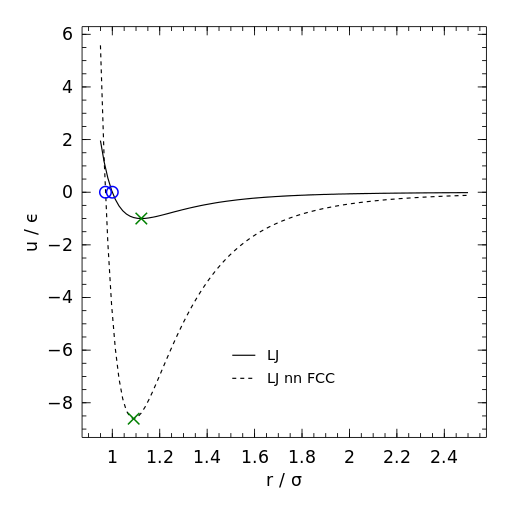
\includegraphics[width=\linewidth]{potentials}
    The LJ potential for a stable crystal structure (FCC) has a deeper potential well, has a longer range attraction, and tends to infinity more quickly when $r \rightarrow 0$.
  \item The LJ potential is given by:
    \begin{equation} \label{eq:LJ}
      u(r) = 4\epsilon\left[\left(\frac{\sigma}{r}\right)^{12} - \left(\frac{\sigma}{r}\right)^{6}\right],
    \end{equation}
    and the LJ potential in a stable, FCC crystal is given by:
    \begin{equation} \label{eq:LJ-FCC}
      U(r_{nn}) = 2\epsilon\left[A_{12}\left(\frac{\sigma}{r_{nn}}\right)^{12} - A_6 \left(\frac{\sigma}{r_{nn}}\right)^{6}\right],
    \end{equation}
    where $A_{12} = 12.13$ and $A_6 = 14.45$.
    Clearly, \eqref{eq:LJ} is equal to zero when $r = \sigma$.
    To find the zero of \eqref{eq:LJ-FCC} we'll use a few steps of algebra:
    \begin{align*}
      0 & = A_{12}\left(\frac{\sigma}{r_{nn}}\right)^{12} - A_6 \left(\frac{\sigma}{r_{nn}}\right)^{6}, \\
      0 & = A_{12}^{1/6}\left(\frac{\sigma}{r_{nn}}\right)^2 - A_6^{1/6} \left(\frac{\sigma}{r_{nn}}\right), \\
      A_6^{1/6} \left(\frac{\sigma}{r_{nn}}\right) & = A_{12}^{1/6}\left(\frac{\sigma}{r_{nn}}\right)^2, \\
      \frac{\sigma}{r_{nn}} & = \left(\frac{A_{6}}{A_{12}}\right)^{1/6}, \\
      r_{nn} & = \sigma \left(\frac{A_{6}}{A_{12}}\right)^{-1/6}, \\
    \end{align*}

    To minimize \eqref{eq:LJ} we'll take the derivative with respect to $r$ and set it equal to zero.
    \begin{align*}
      \frac{du}{dr} = 0 & = 4\epsilon\left[-12 \sigma^{12} r^{-13} + 6 \sigma^6 r^{-7} \right], \\
      0 & = \sigma^6 r^{-7} - 2 \sigma^{12} r^{-13}, \\
      2 \sigma^{12} r^{-13} & = \sigma^6 r^{-7}, \\
      r^{-6} = \frac{1}{2} \sigma^{-6}, \\
      r = \left(\frac{1}{2}\right)^{-1/6} \sigma. \\
    \end{align*}
    Similarly, minimizing \eqref{eq:LJ-FCC} results from:
    \begin{equation*}
      r = \left(\frac{1}{2}\frac{A_6}{A_{12}}\right)^{-1/6} \sigma.
    \end{equation*}
  \item $\frac{\sqrt{\epsilon} k_B}{\sqrt{m}\sigma^2}$.
  \item For argon, the dimensionless temperature is $20 \text{ K} / (\epsilon / k_B) = 0.165$ and the dimensionless thermal conductivity is $1.4 \text{ W} / \text{mK} / \frac{\sqrt{\epsilon} k_B}{\sqrt{m}\sigma^2} = 73.9$.
For krypton, the dimensionless temperature is $0.123$ and the dimensionless thermal conductivity is $106$.
\end{enumerate}

\bibliographystyle{abbrvnat}
\bibliography{master}

\end{document}
